
\section{Overview of Experimental Setup}
All experiments were run on a laptop with an NVIDIA RTX~3050 (4~GB) GPU and 16 CPU threads. The answering
model is \llmName{} in fp16 with greedy decoding; the embedding model is all-MiniLM-L6-v2 and the re-ranker
is the MS~MARCO MiniLM-L6 cross-encoder. Four experiments were carried out:
\begin{enumerate}[nosep]
  \item \textbf{Main comparison} (Section~\ref{sec:main}): five answering strategies on the \nUsers-user,
        \nQuestions-question test split described in Section~\ref{sec:data}.
  \item \textbf{Hallucination analysis} (Section~\ref{sec:halluc}): hallucination rates of every strategy
        and the precision/recall of the grounding gate, compared with the Phase-1 detectors.
  \item \textbf{Retrieval ablation} (Section~\ref{sec:ablation}): each pipeline stage switched on in turn,
        plus pruning and conflict-threshold sweeps, measured with retrieval metrics (no LLM).
  \item \textbf{Context-length scaling} (Section~\ref{sec:niah}): the needle-in-a-haystack protocol of
        Phase 1, now run on our own hardware with histories from 1k to \niahMaxLen{} tokens.
\end{enumerate}
All hyper-parameters were fixed on the separate development split before the test split was evaluated.

\section{Main Comparison of Answering Strategies}
\label{sec:main}
Table~\ref{tab:main} and Figure~\ref{fig:main} summarise the end-to-end results.
\begin{table}[htbp]\centering\small\resizebox{\textwidth}{!}{%
\begin{tabular}{lccccc}\hline
\textbf{Method} & \textbf{Accuracy} & \textbf{Acc. (answerable)} & \textbf{Halluc. rate} & \textbf{Abstain (unans.)} & \textbf{Prompt tokens}\\\hline
Baseline LLM (no memory) & 18.2\% & 0.0\% & 0.0\% & 100.0\% & 117\\
Full context (whole history) & 57.3\% & 61.1\% & 36.1\% & 40.0\% & 4,209\\
Sliding window (last 40 turns) & 26.4\% & 11.1\% & 11.2\% & 95.0\% & 664\\
Vector RAG (Phase-1 design) & 73.6\% & 73.3\% & 17.9\% & 75.0\% & 266\\
\textbf{Memory layer (proposed)} & \textbf{78.2\%} & \textbf{80.0\%} & \textbf{15.5\%} & \textbf{70.0\%} & \textbf{267}\\
\textbf{Memory layer + grounding gate} & \textbf{80.6\%} & \textbf{79.3\%} & \textbf{7.0\%} & \textbf{86.7\%} & \textbf{267}\\
\hline\end{tabular}}
\caption{End-to-end comparison on the long-term conversational memory benchmark (20 users, 330 questions, Qwen2.5-1.5B-Instruct).}
\label{tab:main}\end{table}


\begin{figure}[htbp]\centering
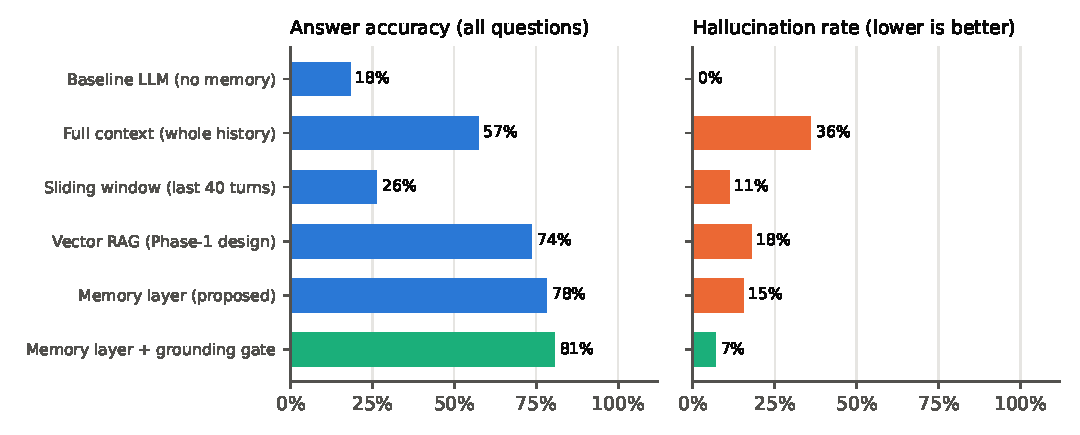
\includegraphics[width=\textwidth]{fig_main_accuracy.pdf}
\caption{Answer accuracy and hallucination rate of the five answering strategies (test split).}
\label{fig:main}
\end{figure}

\textbf{Baseline LLM.} Without any memory the model answers \accNone\% of the questions, and all of those
are unanswerable questions on which it correctly says ``I don't know''. It never guesses a personal fact,
so its hallucination rate is \halNone\%, but it is useless for the task: accuracy on answerable questions
is \accAnsNone\%.

\textbf{Full context.} Sending the entire history (\tokFull{} tokens per query on average) recovers
\accFull\% accuracy, but it also produces the highest hallucination rate of all strategies, \halFull\%. With
288 turns in the prompt, eight of which are distractor facts about other people, the model frequently
returns the neighbour's dog or the colleague's city, and it confuses old and current facts. This is the
Phase-1 finding reproduced with our own model and data: a longer context is not a reliable memory.

\textbf{Sliding window.} The last 40 turns cost \tokWin{} tokens and give only \accWin\% accuracy, because
almost every fact was stated in an earlier session. Its low hallucination rate (\halWin\%) is simply the
result of abstaining most of the time.

\textbf{Vector RAG (Phase-1 design).} Embedding search alone is already a large improvement: \accRag\%
accuracy with \tokRag{} tokens per query, i.e.\ \tokRatioFullMem$\times$ fewer tokens than the full
context and a higher accuracy. Its retrieval recall@5 is \recRag\%.

\textbf{Memory layer.} The full pipeline raises recall@5 to \recMem\% and accuracy to \accMem\%
(\accAnsMem\% on answerable questions) at the same token cost, and lowers the hallucination rate to
\halMem\%. With the grounding gate the hallucination rate halves again to \halMemGate\% while accuracy
rises to \accMemGate\%, because answers copied from a note about the wrong person are converted into
abstentions, which are the correct response for the unanswerable questions (abstention rate
\absMemGate\% versus \absMem\% without the gate).

\section{Accuracy by Question Type}
Table~\ref{tab:types} and Figure~\ref{fig:types} break the accuracy down by question type, which shows
\emph{where} the memory layer differs from plain vector RAG.
\begin{table}[htbp]\centering\small\resizebox{\textwidth}{!}{%
\begin{tabular}{lccccc}\hline
\textbf{Method} & \textbf{Single-hop} & \textbf{Temporal (current)} & \textbf{Temporal (before)} & \textbf{Multi-hop} & \textbf{Unanswerable}\\\hline
Full context (whole history) & 62.4\% & 80.0\% & 13.3\% & 77.5\% & 40.0\%\\
Sliding window (last 40 turns) & 10.0\% & 30.0\% & 0.0\% & 10.0\% & 95.0\%\\
Vector RAG (Phase-1 design) & 80.6\% & 86.7\% & 50.0\% & 50.0\% & 75.0\%\\
Memory layer (proposed) & 81.2\% & 90.0\% & 63.3\% & 80.0\% & 70.0\%\\
\hline\end{tabular}}
\caption{Accuracy by question type.}\label{tab:types}\end{table}


\begin{figure}[htbp]\centering
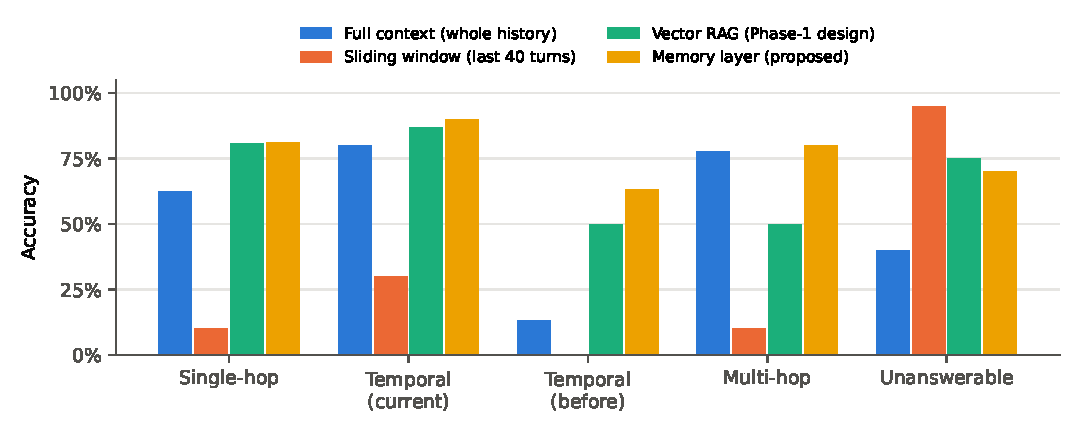
\includegraphics[width=\textwidth]{fig_type_accuracy.pdf}
\caption{Accuracy by question type for the four context-based strategies.}
\label{fig:types}
\end{figure}

\begin{itemize}[nosep]
  \item \textbf{Multi-hop} questions are where the entity graph pays off: \accMemMH\% for the memory
        layer against \accRagMH\% for vector RAG. Vector search finds the note that introduces the
        relative but not the note about that relative, which never mentions the relation word.
  \item \textbf{Temporal (before)} questions improve from \accRagTB\% to \accMemTB\%: the conflict rule
        keeps the old version of a fact in the prompt and tags it as an older note, so the model can
        answer ``where did the user live before moving''. The full-context baseline reaches only
        \accFullTB\% here: with both statements thousands of tokens apart it almost always returns the
        current value.
  \item \textbf{Temporal (current)} questions are answered similarly by the two retrieval methods
        (\accRagTC\% and \accMemTC\%) and by the full context (\accFullTC\%); the chronological rendering
        and the ``trust the most recent note'' instruction already handle most updates.
  \item \textbf{Single-hop} questions are answered correctly \accMemSH\% of the time by the memory layer
        and \accRagSH\% by vector RAG. Retrieval recall is above 97\% for both, so the remaining errors are
        generation errors of the 1.5B model in the presence of distractor notes.
  \item \textbf{Unanswerable} questions are the weak point of every retrieval method without the gate:
        when nothing relevant exists, the retriever still returns five notes and the small model is
        tempted to answer from them. The grounding gate raises abstention on these questions to
        \absMemGate\%.
\end{itemize}

\section{Hallucination Analysis and the Grounding Gate}
\label{sec:halluc}
In Phase 1 the hallucination detectors available for RAG outputs (Table~4.1 of the Phase-1 report)
reached recall of 0.88--0.95 but precision of only 0.25--0.26: they flagged almost everything. The
Phase-2 grounding gate takes the opposite approach. It does not try to judge fluency or plausibility;
it checks three deterministic properties of the answer against the injected notes: is the answer
attributable to a note, is that note a statement rather than a request, and is the note about the same
subject as the question. Table~\ref{tab:halluc} compares the two phases on their respective data.
\begin{table}[htbp]\centering\small
\begin{tabular}{lccc}\hline
\textbf{Detector} & \textbf{Precision} & \textbf{Recall} & \textbf{F1}\\\hline
Phase 1: Mistral 7B (RAGTruth) & 0.25 & 0.92 & 0.39\\
Phase 1: Llama 2 (RAGTruth) & 0.26 & 0.95 & 0.41\\
Phase 1: TinyLlama (RAGTruth) & 0.25 & 0.88 & 0.38\\\hline
Phase 2: grounding gate on vector RAG & 0.89 & 0.42 & 0.57\\
Phase 2: grounding gate on memory layer & 0.93 & 0.55 & 0.69\\
\hline\end{tabular}
\caption{Hallucination detection: Phase-1 results versus the Phase-2 grounding gate.}\label{tab:halluc}\end{table}


On the memory layer's answers the gate flags \gateFlaggedMem{} of \nQuestions{} answers, of which
\gateTPMem{} are indeed hallucinations (precision \gatePMem); it misses \gateFNMem{} of the
\gatePosMem{} hallucinations, mostly answers that copy the \emph{wrong user fact} (e.g.\ the user's
company when asked for the gym), which are attributable, factual and about the user and therefore pass all
three checks (recall \gateRMem). The resulting F1 of \gateFMem{} is substantially above the 0.38--0.41 of the Phase-1
detectors, and, unlike those detectors, the gate costs no additional model call. Applied to the vector-RAG
pipeline the same gate reaches F1 \gateFRag, so the gain is not specific to our retriever.

The hallucination rate of the complete system (memory layer with gate) is \halMemGate\% over all
questions and \halAnsMemGate\% on answerable questions, compared with \halFull\% for the full-context
approach and \halRag\% for plain vector RAG.

\section{Retrieval Ablation}
\label{sec:ablation}
Table~\ref{tab:ablation} and Figure~\ref{fig:ablation} switch the pipeline stages on one at a time and
report retrieval quality on the 270 answerable test questions. Recall@$k$ requires \emph{all} gold
memories of a question to be in the top-$k$ (two for multi-hop questions).
\begin{table}[htbp]\centering\small
\begin{tabular}{lccccc}\hline
\textbf{Configuration} & \textbf{R@1} & \textbf{R@3} & \textbf{R@5} & \textbf{MRR} & \textbf{Temporal ok}\\\hline
Vector only & 58.9\% & 86.3\% & 90.4\% & 0.829 & 70.0\%\\
BM25 only & 24.1\% & 41.1\% & 43.7\% & 0.439 & 26.7\%\\
+ RRF hybrid & 48.9\% & 79.6\% & 87.4\% & 0.756 & 65.0\%\\
+ query exp. & 54.8\% & 80.0\% & 89.6\% & 0.794 & 61.7\%\\
+ re-ranking & 54.1\% & 84.1\% & 88.9\% & 0.801 & 60.0\%\\
+ entity graph & 54.1\% & 84.8\% & 90.7\% & 0.801 & 60.0\%\\
+ scoring (full) & 56.7\% & 88.9\% & 96.3\% & 0.827 & 80.0\%\\
\hline\end{tabular}
\caption{Retrieval ablation: each row adds one stage to the previous one. R@k = all gold memories within the top-k; Temporal ok = the current fact outranks the outdated one.}\label{tab:ablation}\end{table}


\begin{figure}[htbp]\centering
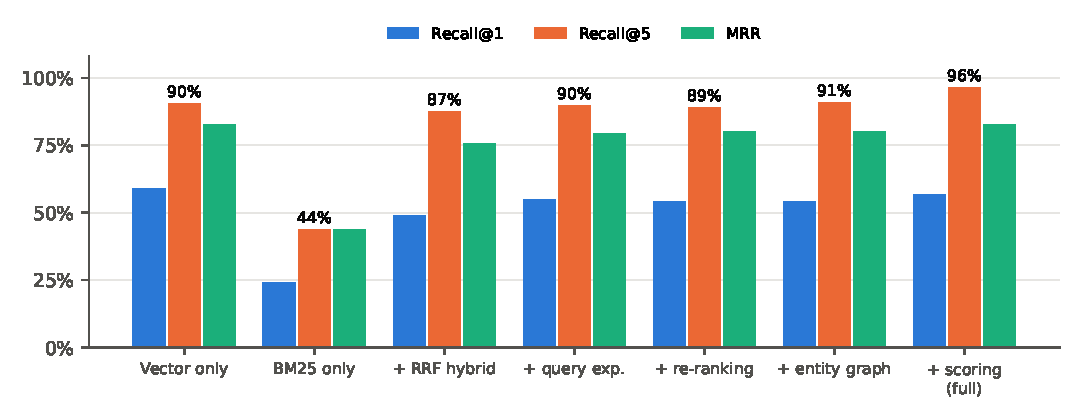
\includegraphics[width=\textwidth]{fig_ablation.pdf}
\caption{Retrieval quality as pipeline stages are added. Each configuration includes all stages to its left.}
\label{fig:ablation}
\end{figure}

\begin{figure}[htbp]\centering
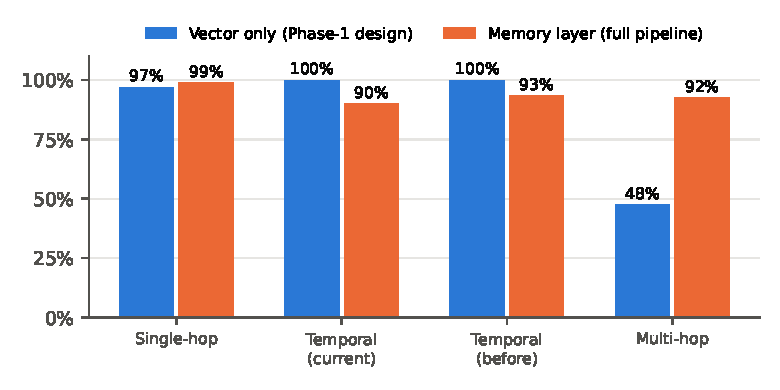
\includegraphics[width=0.78\textwidth]{fig_ablation_types.pdf}
\caption{Recall@5 by question type: Phase-1 vector-only retrieval versus the full memory layer.}
\label{fig:ablation_types}
\end{figure}

Three observations stand out. First, \textbf{BM25 on its own is poor} (\rFiveBm\% recall@5) because the
questions are paraphrases of the stored statements, and fusing the raw lexical ranking with the dense one
\emph{lowers} recall below dense retrieval alone (\rFiveHyb\% vs.\ \rFiveVec\%); only with query
expansion does the lexical channel stop hurting (\rFiveQe\%), and it starts paying off once the later
stages can exploit the exact-match candidates it contributes. Second, the
\textbf{entity graph} is the stage that changes the picture for multi-hop questions:
recall@5 on them goes from \rFiveVecMH\% for vector-only retrieval to \rFiveMemMH\% for the full layer
(Figure~\ref{fig:ablation_types}), with almost no cost on single-hop questions (\rFiveVecSH\% vs.\
\rFiveMemSH\%). Third, \textbf{memory scoring and the question penalty} add the final points: overall
recall@5 rises from \rFiveVec\% (Phase-1 design) to \rFiveMem\%, and the share of temporal questions whose
current version outranks the outdated one rises from \tempVec\% to \tempMem\%.

\section{Importance-Based Pruning and the Conflict Threshold}
\label{sec:pruning}
Table~\ref{tab:pruning} and Figure~\ref{fig:pruning} vary the write-time importance threshold $\theta$.
Keeping only turns with importance $\ge 0.3$ stores \pruneKeptThree\% of the turns and still achieves
\pruneRecThree\% recall@5 (\pruneRecZero\% with everything stored); the discarded turns are generic
assistant replies and short small talk. At $\theta = 0.45$ only \pruneKeptFortyFive\% of the turns remain
for a recall of \pruneRecFortyFive\%, a loss of under four points for a six-fold smaller store, and above
$\theta = 0.5$ genuine facts start to be dropped and recall falls quickly. The importance heuristic
therefore separates facts from chatter well enough to halve the memory store at no cost, and the
threshold gives an explicit storage/recall trade-off.
\begin{table}[htbp]\centering\small
\begin{tabular}{lccc}\hline
\textbf{Importance threshold $\theta$} & \textbf{Memories kept} & \textbf{R@5} & \textbf{MRR}\\\hline
0.0 & 100.0\% & 96.3\% & 0.827\\
0.3 & 55.5\% & 95.9\% & 0.811\\
0.45 & 16.9\% & 92.6\% & 0.779\\
0.55 & 9.6\% & 80.4\% & 0.695\\
0.65 & 6.8\% & 76.3\% & 0.658\\
\hline\end{tabular}
\caption{Write-time pruning: fraction of turns kept as memories and the resulting retrieval quality.}\label{tab:pruning}\end{table}


\begin{figure}[htbp]\centering
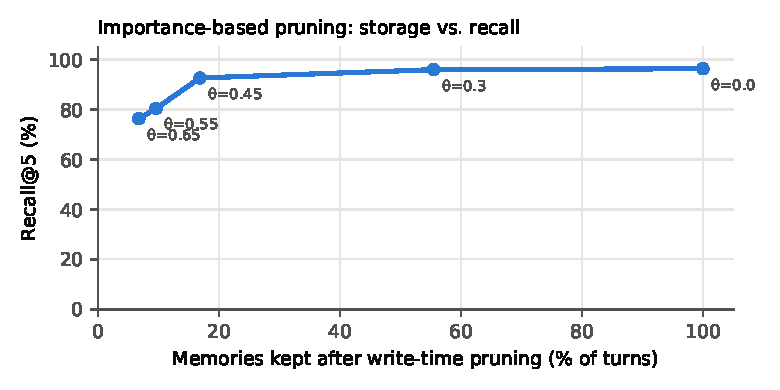
\includegraphics[width=0.72\textwidth]{fig_pruning.pdf}
\caption{Write-time pruning: fraction of turns kept versus retrieval recall for different thresholds.}
\label{fig:pruning}
\end{figure}

The conflict-threshold sweep shows the expected trade-off: a low cosine threshold (0.3) tags more pairs as
old/new versions and gives the best temporal ordering, but also tags unrelated facts and slightly lowers
overall recall; the dev-selected value of 0.45 keeps overall recall at its maximum while still ordering
\tempMem\% of temporal questions correctly.

\section{Context-Length Scaling (Needle in a Haystack)}
\label{sec:niah}
Phase 1 quoted needle-in-a-haystack results from the literature. Here the protocol was run on our own
model: a single personal fact is placed at one of five depths inside a filler conversation of 1k to
\niahMaxLen{} tokens (plus six distractor facts), and the model is asked about it either from the full
transcript or from the memory layer's top-5 notes (\niahNeedles{} needles per cell, \niahCells{} cells).
Table~\ref{tab:niah} and Figures~\ref{fig:niah} and~\ref{fig:niah_heat} give the results.
\begin{table}[htbp]\centering\small
\begin{tabular}{lcccccc}\hline
\textbf{History length} & \multicolumn{3}{c}{\textbf{Full context}} & \multicolumn{3}{c}{\textbf{Memory layer}}\\
 & Acc. & Tokens & Latency & Acc. & Tokens & Latency\\\hline
1k & 82\% & 1,080 & 1.11s & 90\% & 270 & 0.65s\\
2k & 82\% & 2,096 & 1.85s & 92\% & 265 & 0.66s\\
4k & 85\% & 4,184 & 3.03s & 80\% & 264 & 0.68s\\
8k & 75\% & 8,335 & 6.23s & 82\% & 263 & 0.67s\\
16k & 75\% & 16,634 & 81.64s & 72\% & 267 & 0.70s\\
\hline\end{tabular}
\caption{Needle-in-a-haystack scaling: accuracy, prompt size and latency versus history length.}\label{tab:niah}\end{table}


\begin{figure}[htbp]\centering
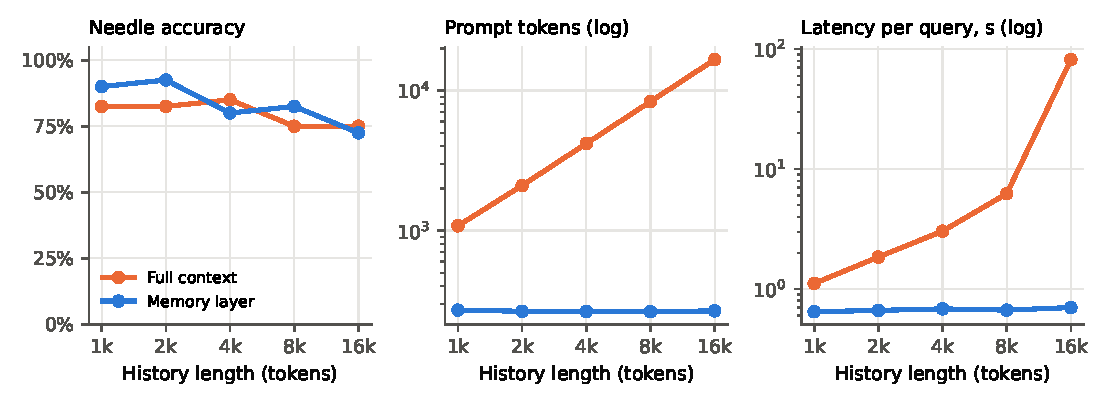
\includegraphics[width=\textwidth]{fig_niah_lines.pdf}
\caption{Needle accuracy, prompt size and latency versus history length for full-context prompting and
the memory layer.}
\label{fig:niah}
\end{figure}

\begin{figure}[htbp]\centering
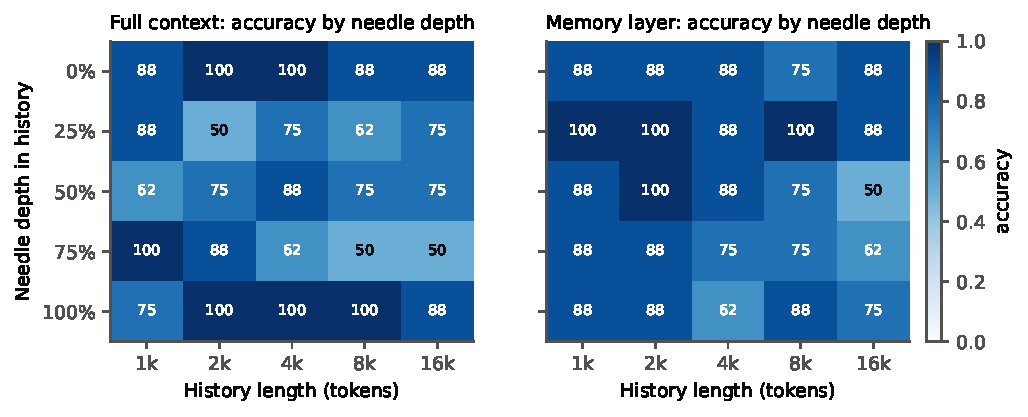
\includegraphics[width=\textwidth]{fig_niah_heatmap.pdf}
\caption{Accuracy by needle depth and history length (the Phase-2 counterpart of the Phase-1 NIAH heatmap).}
\label{fig:niah_heat}
\end{figure}

Two things are visible. The memory layer's prompt stays at about \niahTokMemLast{} tokens whatever the
history length, while the full-context prompt grows to \niahTokFullLast{} tokens at \niahMaxLen{}
(\niahTokRatioLast$\times$ more); latency grows accordingly, from \niahLatFullFirst{}~s to
\niahLatFullLast{}~s per query for the full context against \niahLatMemLast{}~s for the memory layer at
\niahMaxLen{} tokens (\niahLatRatioLast$\times$ faster). On this single-needle task the 1.5B model's
accuracy from the full context is \niahFullAccFirst\% at 1k and \niahFullAccLast\% at \niahMaxLen{}
tokens (mean \niahFullAccMean\%), while the memory layer gives \niahMemAccFirst\% and \niahMemAccLast\%
(mean \niahMemAccMean\%) with the needle retrieved into the top-5 in \niahMemRecallMean\% of cases.
At \niahMaxLen{} tokens the memory layer holds \niahMemMemories{} notes; the needle is still retrieved
93\% of the time, so its lower accuracy there is again a reading error of the small model, which has to
pick the needle out of five notes that now include more same-attribute distractors.
The important contrast with Section~\ref{sec:main} is that a \emph{single} needle in filler text is a
much easier problem than a real multi-session history: the full-context model degrades far more when the
haystack contains many similar facts, updates and distractors (\accFull\% there) than when it contains
one fact among small talk. The difficulty of long-context memory is interference, not length alone, and
retrieval of a few verified notes removes the interference while keeping the cost constant.

\section{Efficiency: Tokens and Latency}
Figure~\ref{fig:tokens} compares prompt size and end-to-end latency on the main benchmark. The memory
layer sends \tokMem{} tokens per query against \tokFull{} for the full context
(\tokRatioFullMem$\times$ fewer) and answers in \latMem{}~s against \latFull{}~s
(\latRatioFullMem$\times$ faster). The retrieval stages themselves (embedding the question, FAISS and
BM25 look-ups, graph expansion, cross-encoder re-ranking and scoring) take 30--50~ms per query on the
GPU and about 30~ms on the CPU, against 6~ms for plain vector search; the rest of the latency is LLM
generation. Ingesting a complete 288-turn history (normalisation, embedding, indexing and entity
extraction) takes well under a second, and a 1,118-note history about a quarter of a second.

\begin{figure}[htbp]\centering
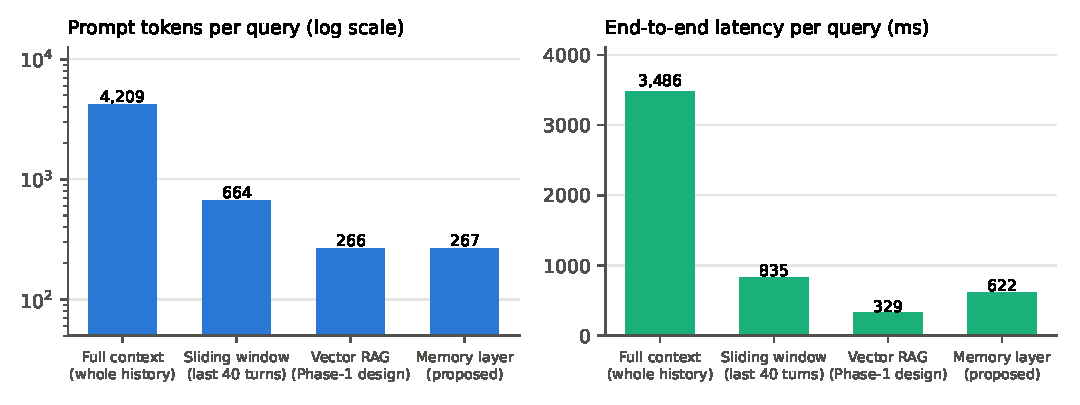
\includegraphics[width=\textwidth]{fig_tokens_latency.pdf}
\caption{Prompt tokens and end-to-end latency per query on the main benchmark.}
\label{fig:tokens}
\end{figure}

\section{Qualitative Example}
Listing~\ref{lst:trace} shows an actual trace of the memory layer on a short three-session history
(run on the CPU, hence the higher latencies). Note the third-person normalisation of the stored notes, the
``(older note)'' tag on the superseded city, the second-hop note (``Priya adopted a cat \dots'') reached
through the entity \emph{Priya}, and the abstention produced by the gate when the model answers the
car question from the note about the colleague. The second question also shows the typical residual error
of the small model: both the old and the new city are in the prompt, correctly labelled, yet it answers
with the current one.
\lstinputlisting[caption={Trace of the memory layer on a three-session history (verbatim program output).},
  label={lst:trace}]{example_trace.txt}

\section{Key Insights}
\begin{itemize}[nosep]
  \item A long context window is the \emph{worst} memory in the presence of updates and distractors: the
        full-context baseline hallucinates \halFull\% of the time, more than any other strategy.
  \item Selective retrieval is the main source of the gain (vector RAG alone reaches \accRag\%); the
        additional stages of the memory layer matter for the question types that vector search cannot
        solve: multi-hop (\accRagMH\% $\rightarrow$ \accMemMH\%) and temporal-before
        (\accRagTB\% $\rightarrow$ \accMemTB\%).
  \item Verification is as important as retrieval: the grounding gate halves the hallucination rate
        (\halMem\% $\rightarrow$ \halMemGate\%) with precision \gatePMem, where the Phase-1 detectors had
        precision 0.25.
  \item Memory can be pruned at write time: half of the turns carry all of the recall, and a sixth of
        them carry 96\% of it.
  \item The remaining errors are mostly generation errors of the small model, not retrieval errors
        (recall@5 \recMem\% versus accuracy \accMem\%), which points to a larger answering model or a
        reader fine-tuned on memory notes as the next step.
\end{itemize}
